\documentclass{article}

\usepackage{natbib}
\usepackage{algorithm}
\usepackage{algorithmic}
\usepackage{amsmath}
\usepackage{geometry}
\usepackage{verbatim}
\usepackage{tabularx}
\usepackage{graphicx}
\usepackage{amsfonts} % just for the indicator variable \mathbb{I}

\title{Elo-R Competition Rating System}
\author{Aram Ebtekar}
\date{April 11, 2016}

\begin{document}
\maketitle

\section{Introduction}

This paper describes the Elo-R rating system, designed for use in programming competitions. In Section 1, we derive the algorithm from Bayesian first principles, as an approximate posterior belief distribution. In Section 2, we justify the algorithm by more intuitive means. We ultimately end up with exactly the same algorithm, so the reader who is less interested in theoretical justifications may skip directly to Section 2.

The "R" in the name may stand for "Ranked", as it operates on game outcomes given as a rank-ordered list of players; or it may stand for "Robust", as the system is designed to be robust to outlier performances, like someone having an off day.

Competitions, in the form of sports, games and examinations, have been with us since antiquity. Whether the purpose is entertainment, training, or selection for a particular role, contestants and spectators alike are interested in estimating the relative skills of contestants. Various competition formats, such as tournaments, exist to declare a champion. However, we may be interested in comparing players who rarely, if ever, play directly against one another. When there is substantial variance in a player's performance, we may be interested in an aggregate estimate of skill based on the player's entire history of games.

Skills are easiest to compare when there is a standard quantifiable objective, such as a score on a standardized test or a completion time in a race.  However, most team sports, as well as games such as chess, have no such measure. Instead, a good player is simply one who can frequently win against other good players. The Elo rating system assigns a quantitative measure of skill in such a scenario. Typically, an average player is  rated 1500, while a top player may exceed 2500. The scale is arbitrary, but can be used to rank players relative to one another, as well as to forecast the probable outcome of future matches.

To make things concrete, let's label the players $1,\ldots,N$. The original Elo system deals with 1v1 zero-sum games with binary (win/lose) outcomes. Player $i$ has a rating $r_i$, a real number that should be higher the more skilled they are. After two players compete, the loser gives some number of points to the winner, so that the sum of ratings is conserved. The number of points transferred depends on how ``surprising" the outcome was. To determine the level of surprise, we need some model of the likelihood of match outcomes between players of known ratings. The logistic function is a common and well-studied choice: in this model, the outcome probability decays exponentially with the rating difference between the losing and winning player.

Elo, and variants such as Glicko \cite{glicko}, are popular choices in the 1v1 setting where each match has a winner and loser. While Elo is not the most accurate predictor of future outcomes, it's accurate enough and has other good properties: the incremental update following each match is simple, fast, and only affects the ratings of participants. Now let's consider a more general setting in which an arbitrary number of players compete simultaneously at a task. The outcome is a ranking, i.e., a total order among all players in the match. That is, we recognize which player came in 1st place, 2nd, 3rd, etc. We ignore the relative margins of victory, as they depend on details of the game that may be difficult to model: if the number of players is sufficiently large, differences in ordinal ranking should encapsulate most of the information about margins of victory.

This model is used in the programming competition websites Codeforces \cite{Codeforces} and TopCoder \cite{TopCoder}, each of which has tens of thousands of rated members from across the globe. Each publishes its own rating system, but without much theoretical justification to accompany the derivations. By founding Elo-R upon a more rigorous probabilistic model, we achieve better properties in practice as well. Compared with the Codeforces system, Elo-R achieves faster convergence, more robustness against unusual performances, and less inflation. Compared with the TopCoder system, Elo-R is more robust against unusual performances, and monotonic in the sense that performing better in a match will never result in a lower rating. The non-monotonicity of TopCoder has been studied in the analysis of \cite{forivsektheoretical}. Furthermore, Elo-R retains simplicity and efficiency roughly on par with the other systems.

In section 2, we describe Elo-R ratings as a weighted average of past performances, with weights depending on the age of the performance and how atypical it is. In section 3, we develop a Bayesian model of contest performance, and use it to derive the Elo-R system, which turns out to match the weighted average discussed previously. Then in section 4, we fill in the remaining details and parameters. In section 5, we discuss some of the system's theoretical and empirical properties, robustness in particular. Finally, section 6 concludes with a summary of how the system might be useful.

\section{Performance Averaging}

Recall that the outcome of a match consists of a total order ranking among all participating players. To model how the outcome came about, suppose player $i$'s true (unknown) skill is $s_i$. Player $i$'s performance in the match can be viewed as a number $p_i$, drawn from a logistic distribution centered at $s_i$. If $i$ beat $j$ in the match rankings, a result we denote as $i \succ j$, then we know that $p_i > p_j$. Note that the event $p_i = p_j$ has probability zero. In practice, some games allow ties. In order to sidestep the issue of modeling ties separately, we will simply treat them as half a win and half a loss; such a division will be very straightforward with the formulas we'll get.

While we can't measure $s_i$ directly, we can estimate $p_i$ by looking at the ratings of other players and at $i$'s position in the ranking. This suggests the following two-phase approach: from the match ranking, estimate $p_i$ for each player. Then, update the rating $r_i$ to a weighted average of past $p_i$s. Note that $s_i,p_i,r_i$ are all measured on a common scale. As we'll soon see, less weight will be put on performances that are either outdated or unusual for the player.

Let's focus on the second phase for now: having computed the latest $p_i$, we want to combine it with past performances of the same player to get a more precise estimate of their skill. To clarify the notation in this section, we add an extra subscript $k$, ranging from $1$ to the number of matches $M$ in which player $i$ has competed, so that $p_{i,k}$ denotes the performance of player $i$ on their $k$th match, and $r_{i,k}$ denotes their rating upon completion of the $k$th match. The sample mean is perhaps the most obvious statistic to take. That is, let
\begin{align}
r_{i,M} = \frac{1}{M} \sum_k p_{i,k} = \left(1 - \frac{1}{M}\right) r_{i,M-1} +  \frac{1}{M} p_{i,M}
\end{align}

In addition to being simple, this method has the advantage of being a function of only the number of matches $M$, the previous rating $r_{i,M-1}$ and the new performance $p_{i,M}$, so there is no need to remember all of the $p_{i,k}$. We say that such a method is \emph{memoryless}.

However, there are two key problems here. The first is that, as a player accumulates more experience, the relative weight of a new performance approaches zero; if an established player improves their skill, it will take a long time for their rating to reflect it. This is because all performances are weighted equally, even those which are too outdated to accurately reflect a player's current skill. The method would be more suitable if a player's true skill were an eternal constant, never changing, and each $p_{i,k}$ were a measurement of this constant. To properly account for a player's lifelong evolution, we should place less weight on older performances.

The second problem with the sample mean is lack of robustness against outliers. A single extreme performance, perhaps due to illness or a power failure (if the competition takes place over a web server), will drastically affect a player's rating. Thus, we wish to reduce the weight of outliers.

Before we proceed, note that the above equation can be rewritten as
\begin{align}
\sum_k w_k(p_{i,k} - r_{i,M}) = 0
\end{align}
where $w_k = 1$ for all $k$. We say that $r_{i,M}$ is a \emph{weighted mean} of the elements $\{p_{i,k}\}_{k=1}^{M}$ with corresponding weights $\{w_k\}_{k=1}^M$. As a simplifying assumption, let's imagine the $p_{i,k}$ are independent measurements of the present true skill $s_{i,k}$, with Gaussian (normal) noise variances of $\tau_k^2$. If we treat $p_{i,1}$ as the prior, then our posterior belief on the true skill is a normal distribution centered at the weighted mean $r_{i,M}$ given by the following equation:
\begin{align}
\sum_k \frac{1}{\tau_k^2} (p_{i,k} - r_{i,M}) = 0
\end{align}

All we did here is set $w_k = 1/\tau_k^2$. If the $w_k$s (or equivalently, the $\tau_k$s) form a geometric sequence, we maintain the memoryless property. We'll derive the weights later; for now, it's simplest to imagine them decreasing by a constant ratio for each match backward in time.

In order to bound the effect of any individual outlier, we also require that $w_k|p_{i,k}|$ approach a positive constant as $p_{i,k}$ approaches $\pm\infty$. We still want to treat non-outliers in essentially the same way as before, so their weight should be close to $1/\tau_k^2$ for performances close to the weighted mean, which is $r_{i,M}$ by definition. To meet these criteria, we opt for
\begin{align}
w_k = \frac{1}{\tau_k(p_{i,k} - r_{i,M})} \tanh\frac{p_{i,k} - r_{i,M}}{\tau_k}
\end{align}

This choice will be justified by a proper derivation later: essentially, it comes from modeling performances according to the heavy-tailed logistic distribution in place of the Gaussian noise discussed previously. Heavier tails are more forgiving of outliers. Substituting (4) into (2), the equation defining $r_{i,M}$ becomes:
\begin{align}
\sum_k \frac {1}{\tau_k} \tanh\frac{p_{i,k} - r_{i,M}}{\tau_k} = 0
\end{align}

It is monotonic in $r_{i,M}$, so it can be solved using binary search. A straightforward linear approximation shows that in the limit as the performances vary much less than any of the $\tau_k$, the rating behaves like a mean with weights $1/\tau_k^2$. In the limit as the performances vary much more than any of the $\tau_k$, the rating behaves like a median with weights $1/\tau_k$. While this equation is not memoryless, all $\tau_k$ corresponding to old performances will be very large, so their terms will behave like their linear approximations. Any sum of linear terms is itself linear, so we can merge the old terms. $p_{i,0}$ here is the weighted sum of the old performances, and the merged weight $1/\tau_0^2$ is the sum of the weights of these old performances. $k$ now ranges only over indices of the new, unmerged, performances:
\begin{align}
\frac{p_{i,0} - r_{i,M}}{\tau_0^2} + \sum_k \frac {1}{\tau_k} \tanh\frac{p_{i,k} - r_{i,M}}{\tau_k} = 0
\end{align}

As a result, we only need to remember a small number of recent performances. Instead of growing without bound with the size of the history, the number of terms in the sum can be set to a small constant while merging the rest. If we decide to remember zero performances, it reverts to the linear memoryless method. Hence, this general formula encapsulates everything we've covered thus far. For greater accuracy, it's best to remember at least a few performances. We will see that (6) is equivalent to maximizing the product of a collection of normal and/or logistic probability density functions (pdfs). $\tau_k^2$ corresponds roughly to the pdf's variance, although it differs by slightly different constant factors for the normal and the logistic; we choose to stick to this parametrization in order to maintain the equivalence involved in the linear approximation.

\section{Bayesian Model}

Now we derive the rating algorithm in full, beginning with a Bayesian model. If a player's true skill is $s_i$, it makes sense to set their rating $r_i$ to our best estimate of $s_i$, given all the evidence from past matches. Our belief on $s_i$ is given by a pdf $f(s_i)$ which changes in response to the evolution of $s_i$ or new evidence $e$. In general, $f(s_i)$ will be proportional to a product of normal and logistic pdfs. We may think of one of the constituent pdfs as a prior belief, and the others as likelihoods of evidence consisting of independent measurements of $s_i$. The rating $r_i$ is then defined as the \emph{maximum a posteriori} (MAP, a.k.a. posterior ``mode") estimate of $s_i$:
\begin{align}
r_i = \arg\max_{s_i} f(s_i\mid e)
\end{align}

\begin{center} 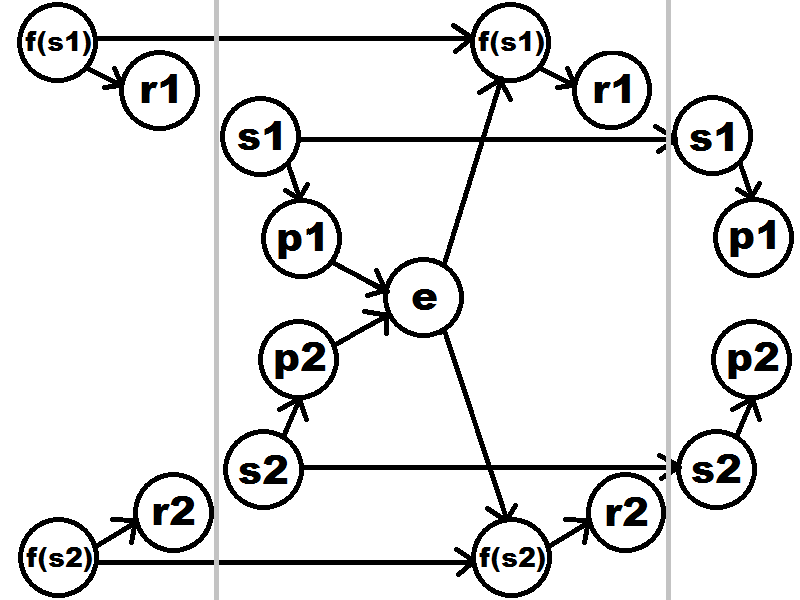
\includegraphics[scale=0.35]{../images/HMMlabeled.png} \end{center}

Our model is essentially a Hidden Markov process. The above figure illustrates a slice of the causal network corresponding to a match with two participants; the match itself is bounded by gray lines, with a few predecessor and successor nodes included for clarity. Each player $i$ performs at level $p_i$, drawn independently from a logistic distribution centered at $s_i$. The values of $s_i$ and $p_i$ are hidden. The observable evidence $e$ is a ranking of all the $p_i$s, i.e., a total ordering of the players based on their performances: $i$ outranks $j$, written $i \succ j$, iff $p_i > p_j$. In the two-player example, this simply tells us which player won. Note that we discard additional information about player scores, which are difficult to model and depend heavily on the specifics of the contest.

In the rest of this paper, we explain how the evidence $e$ is used to update the belief. In fact, the nodes labeled $f(s_i)$ correspond to all of the information that we choose to keep for belief computation purposes. This information is summarized by publishing a numerical rating $r_i = \arg\max_{s_i} f(s_i\mid e)$. Between this match and the next one, the player's skill $s_i$ may improve or decline. Therefore, the figure includes additional $s_i$ and $p_i$ nodes on the right; the next match may reveal a ranking amongst these and other $p_i$s from all players who choose to participate.

In practice, we make a few approximations. Fix $i$, the player whose rating we presently compute. Let $e$ be the evidence consisting of, for each $j$, whether $i \succ j$ or $i \prec j$. That is, we ignore relations like $j \succ k$ which affect the relative ordering of player pairs that don't include $i$. Our goal is to approximate the posterior distribution of $s_i$ given $e$:
\begin{align}
f(s_i\mid e) \propto f(s_i)\Pr(e\mid s_i) = f(s_i)\int \Pr(e\mid p_i)f(p_i\mid s_i)dp_i
\end{align}

Since the integral is hard to evaluate, we take a leap of faith here and treat $\Pr(e\mid p_i)$ as a (possibly scaled) delta-function that spikes at the MAP estimate of $p_i$. This is justified as $N \rightarrow \infty$, because the evidence $e$ would overwhelmingly concentrate $p_i$ into a narrow range. Having fixed $p_i$, the previous equation simplifies to
\begin{align}
f(s_i\mid e) \propto f(s_i)f(p_i\mid s_i)
\end{align}

Our update algorithm thus divides into two phases: first, it must determine the player's performance $p_i$ in the match. In the second phase, $p_i$ is used to update the belief distribution on $s_i$, which is then compactly summarized by finding the point $r_i$ that achieves its maximum.

\subsection{Performance Estimation}

To compute the MAP of $p_i$, we must maximize
\begin{align}
f(p_i\mid e) \propto f(p_i) \Pr(e\mid p_i)
\end{align}

Clearly, $p_i = r_i + (s_i-r_i) + (p_i-s_i)$. The first term is a known constant: the player's current rating. We have a prior belief on $s_i$; we'll eventually see it has a fairly general form but, for the purposes of this phase, we approximate it by a logistic random variable with mean $r_i$. We also modeled $p_i$ as a logistic random variable centered at $s_i$. Hence, the second and third terms have mean zero and known variance.

If we approximate the random terms by normal random variables, then their sum is conveniently also normal with a straightforward mean and variance. However, since the terms were originally logistic, we model their sum as another logistic variable with this mean and variance. To make things concrete, the model I implemented for Codeforces has the parameters $\sigma_i = 100$ (by default, but see discussion of new players), $\delta = 250$, and $\delta_i^2 = \sigma_i^2 + \delta^2$. The corresponding logistic pdfs are:
\begin{align}
f(s_i) \approx \frac { 2e^{2(s_i-r_i)/\sigma_i} } { \sigma_i\left(1 + e^{2(s_i-r_i)/\sigma_i} \right)^2 }
\\f(p_i\mid s_i) = \frac { 2e^{2(p_i-s_i)/\delta} } { \delta\left(1 + e^{2(p_i-s_i)/\delta} \right)^2}
\\f(p_i) \approx \frac { 2e^{2(p_i-r_i)/\delta_i} } { \delta_i\left(1 + e^{2(p_i-r_i)/\delta_i} \right)^2}
\end{align}

Under these modeling assumptions,
\begin{align}
\Pr(e\mid p_i) &= \prod_{j \succ i} \Pr(p_j > p_i) \prod_{j \prec i} \Pr(p_j < p_i)
\\&\approx \prod_{j \succ i} \frac {1} {1 + e^{2(p_i-r_j)/\delta_j}} \prod_{j \prec i} \frac {e^{2(p_i-r_j)/\delta_j}} {1 + e^{2(p_i-r_j)/\delta_j}}
\\&\propto \frac {e^{2p_i\sum_{j\prec i}1/\delta_j}} {\prod_{j\neq i} 1 + e^{2(p_i-r_j)/\delta_j}}
\end{align}

Taking logarithms, there exist a constant $C$ such that
\begin{align}
C + \ln f(p_i\mid e) &= \ln f(p_i) + \ln \Pr(e\mid p_i)
\\&\approx \ln \frac{2}{\delta_i} + (p_i-r_i)\frac{2}{\delta_i} - 2\ln\left(1 + e^{2(p_i-r_i)/\delta_i} \right) + 2p_i\sum_{j\prec i} \frac{1}{\delta_j} - \sum_{j\neq i} \ln\left(1 + e^{2(p_i-r_j)/\delta_j}\right)
\end{align}

To maximize this expression, differentiate it w.r.t. $p_i$, divide by 2 and set to zero:
\begin{align}
0 &= \frac{1}{\delta_i}\left(1 - \frac {2e^{2(p_i-r_i)/\delta_i}} {1 + e^{2(p_i-r_i)/\delta_i}} \right) + \sum_{j\neq i}\frac{1}{\delta_j}\left(\mathbb{I}(j\prec i) - \frac {e^{2(p_i-r_j)/\delta_j}} {1 + e^{2(p_i-r_j)/\delta_j}} \right)
\\&= \sum_{j\preceq i}\frac{1}{\delta_j}\left(\frac {1} {1 + e^{2(p_i-r_j)/\delta_j}} \right)
	- \sum_{j\succeq i}\frac{1}{\delta_j}\left(\frac {e^{2(p_i-r_j)/\delta_j}} {1 + e^{2(p_i-r_j)/\delta_j}} \right)
\\&\propto \sum_{j\preceq i}\frac{1}{\delta_j}\left( \tanh\frac {p_i - r_j} {\delta_j} - 1 \right) + \sum_{j\succeq i}\frac{1}{\delta_j}\left( \tanh\frac {p_i - r_j} {\delta_j} + 1 \right)
\end{align}

Use binary search to solve for $p_i$. This defines the \emph{performance} of player $i$ in the match.

The terms in parentheses can be thought of as a measure of surprise at the outcomes between $i$ and $j$: they are the probability of the outcomes opposite to what actually occurred, when the performance of player $i$ is fixed to $p_i$. In addition to the actual outcomes, the sum also contains two artificial outcomes in which player $i$ wins once and loses once (or equivalently, ties twice) against clones of itself. These regularizing outcomes come from the prior, and prevent the first- and last-place players from achieving $p_i = \pm\infty$. The equation chooses $p_i$ in such a way that the total surprise from wins is equal to the total surprise from losses.

For a more intuitive interpretation, note that if the $\delta_j$s were all equal, this amounts to finding the performance level $p_i$ at which one's expected rank would match player $i$'s actual rank, clones included.

\subsection{Posterior Maximization}

Recall our approximation $f(s_i\mid e) \propto f(s_i)f(p_i\mid s_i)$: the posterior $f(s_i \mid e)$ takes the prior $f(s_i)$ and multiplies it by a new logistic pdf $f(p_i\mid s_i)$. It will inductively be the case that our posterior is proportional to a product of normal and logistic pdfs. Since any product of normal pdfs has a normal kernel, WLOG we can assume there is only one normal in the product:

\begin{align}
f(s_i\mid e) \propto e^{-(s_i-\mu_0)^2/\tau_0^2} \prod_k \frac { e^{2(s_i-\mu_k)/\tau_k} } { \left(1 + e^{2(s_i-\mu_k)/\tau_k} \right)^2 }
\end{align}

\begin{align}
C + \ln f(s_i \mid e) &= -\frac{(s_i-\mu_0)^2}{\tau_0^2} + 2\sum_k \left( \frac{s_i-\mu_k}{\tau_k} - \ln(1 + e^{2(s_i-\mu_k)/\tau_k}) \right)
\end{align}

We will discuss the parameters $\mu_k$ and $\tau_k^2$, which correspond roughly to mean and variance of the corresponding pdfs, in the next section. To maximize $\ln f(s_i \mid e)$ after being given these parameters, differentiate it w.r.t. $s_i$, divide by 2 and set to zero:
\begin{align}
0 &= \frac{\mu_0-s_i}{\tau_0^2} + \sum_k \frac{1}{\tau_k}\left( 1 - \frac {2e^{2(s_i-\mu_k)/\tau_k}} {1 + e^{2(s_i-\mu_k)/\tau_k}} \right)
\\0 &=  \frac{\mu_0-s_i}{\tau_0^2} + \sum_k \frac{1}{\tau_k} \tanh \frac {\mu_k-s_i} {\tau_k}
\end{align}

Solve for $s_i$ using binary search: this is the MAP estimate we will use as the new rating $r_i$. When the $\mu_k$s are the performances of player $i$ in previous matches, this is identical to the weighted mean from equation (6). If time and memory are a concern, we can apply the same trick to merge old tanh terms (i.e. indices $k$ for which $\tau_k$ is large) into the normal term.

If all but the last $M$ matches for each player are merged, and all binary searches are performed to an accuracy of $\epsilon$, then a match with $N$ players is processed in $O((N^2+NM)\log(1/\epsilon))$ time. The ratings accumulate $O(\epsilon)$ numerical error per match, and likely a lot less in the long run due to statistical averaging. The Elo-R update is summarized in Algorithm \ref{alg:update}. It's easy to see that the loops and summations are highly parallelizable.

\section{Noise, Uncertainty, and Evolution}

We now know how to compute $p_i$ from a match's rankings, and how to compute $r_i$ from the general form of the posterior belief over $s_i$. It remains to link these steps by building the posterior belief corresponding to a history of $p_i$s. For new players, we can consider assigning either a logistic or normal prior. Since we want fast convergence, but also believe that extremely high ratings should take time to earn, we opt for a normal prior with $\mu_0 = 1500$ and $\tau_0 = 350$. We can think of this as the ``posterior" belief in any player's skill upon completing zero matches.

In the general case, we wish to go from the posterior distribution after $M-1$ matches, which we'll denote by $f'(s_i)$; to the prior distribution just before the $M$th match, denoted by $f(s_i)$; and finally to the posterior distribution after the $M$th match, denoted by $f(s_i \mid e)$. Here $e$ denotes the evidence from the $M$th match.

As previously discussed, we need to model changes in a player's skill between matches. Although $f'(s_i)$ and $f(s_i)$ are based upon the same body of evidence, they are not identical: $f(s_i)$ has more uncertainty because $s_i$ was changed by a noise term in the interim between the two matches. Once we have $f(s_i)$, estimating $f(s_i \mid e)$ is a simple matter of multiplying $f(s_i)$ by $f(p_i \mid s_i)$. The latter is a logistic term with $\mu_k = p_i,\;\tau_k=\delta$, where $p_i$ is computed as above and $\delta$ is a specified constant.

How should we model the increase in uncertainty between $f'(s_i)$ and $f(s_i)$? It can be shown that a product of normal pdfs with variances $\{\sigma_k^2\}$ corresponds to a normal with variance $1/(\sum_k 1/\sigma_k^2)$. While general products of probability distributions don't have this property, let's define by analogy the \emph{uncertainty} of our normal-logistic product beliefs to be $1/(\sum_k 1/\tau_k^2)$. Recall when we introduced the constant $\sigma_i$ to represent the uncertainty in our belief. With our new definition of uncertainty, $\sigma_i$ is no longer a constant but is instead given by:
\begin{align}
\frac{1}{\sigma_i^2} &= \sum_k \frac{1}{\tau_k^2}
\end{align}

When we multiply $f(s_i)$ by the logistic pdf $f(p_i \mid s_i)$, the latter corresponds to new information about $s_i$. Here, the term \emph{information} refers to the reciprocal of uncertainty. If we continue to add information, the uncertainty will tend toward zero. As discussed in the first section, we must prevent this in order to respond to a player's evolution over time. To this end, let's say $s_i$ changes between matches by a noise term centered at $0$ with uncertainty $\eta^2$. If we want the amount of noise to increase with physical time, we could model it as Brownian motion. I chose instead to add a constant lump term right before each match.

Thus, $s_i$ after the $M$th match is equal to $s_i$ before the match, plus a noise term. Deriving $f(s_i)$ from $f'(s_i)$ amounts to accounting for this noise. A crude way to approximate its effect would be to increase all of the $\tau_k$. If we want the weight of old matches to decay exponentially in some natural limiting cases, then it makes sense to multiply all of the $\tau_k$ by the same constant $K$. Furthermore, in analogy to additivity of variances in response to a random noise offset, $K$ should be chosen in such a way that the belief uncertainty is increased by $\eta^2$. Thus, if $f'(s_i)$ has a factor with uncertainty $\tau_k$, then $f(s_i)$ has the same factor but with its uncertainty changed to $K\tau_k^2$ where:
\begin{align}
\frac{1}{\sum_k 1/(K\tau_k^2)} &= \frac{1}{\sum_k 1/\tau_k^2} + \eta^2
\\ \text{Therefore, }K &= 1 + \eta^2\sum_k 1/\tau_k^2
\end{align}

The noise constant $\eta$ is chosen such that $\sigma_i$ approaches the limiting constant $\sigma^*$ as the number of matches goes to infinity. Setting $1/\sigma_i^2$ to $1/\sigma^*$ both before and after the match yields the fixpoint equation:

\begin{align}
\frac{1}{\sigma^{*2}} &= \frac{1}{\sigma^{*2} + \eta^2} + \frac{1}{\delta^2}
\\ \text{Therefore, }\eta^2 &= \frac{1}{1/\sigma^{*2} - 1/\delta^2} - \sigma^{*2}
\end{align}

My Codeforces model uses $\delta = 250$ and $\sigma^* = 100$, yielding a noise of $\eta \approx 43.64$. The uncertainty $\sigma_i$ for a new player is 350, which asymptotically approaches $\sigma^* = 100$ as they gain experience. The parameter and prior belief initializations are summarized in Algorithm \ref{alg:init}. Note that the first element in a player's list of pdf belief factors corresponds to the normal factor contributed by the prior and old merged performances, while the tail of the list are logistic factors corresponding to increasingly recent performances.

In order to give new players lower ratings from which to work upwards, we can publish $r_i - 2(\sigma_i - \sigma^*)$, rounded to the nearest integer, as the official rating instead of $r_i$. Thus, a new player's published rating is $1500 - 2(350-100) = 1000$. As the difference term vanishes, an experienced player's published rating becomes very close to $r_i$.

\begin{algorithm}
\caption{$init()$}
\label{alg:init}
\begin{algorithmic}
\STATE $\sigma^* := 100$
\STATE $\delta := 250$
\STATE $\eta^2 := 1 / \left( 1/\sigma^{*2} - 1/\delta^2 \right) - \sigma^{*2}$
\FORALL{players $i$}
\STATE Initialize the list $\langle( \mu_{i,\_},\tau_{i,\_} )\rangle$ with one element $(1500, 350)$
\STATE $r_i := 1500$
\STATE $\sigma_i := 350$
\STATE $\delta_i := \sqrt{\sigma_i^2 + \eta^2 + \delta^2}$
\ENDFOR
\end{algorithmic}
\end{algorithm}

\begin{algorithm}
\caption{$update()$}
\label{alg:update}
\begin{algorithmic}
\FORALL{match participants $i$}
\STATE $p_i := $ SOLVE $\sum_{j\preceq i}\frac{1}{\delta_j}\left( \tanh\frac {p_i - r_j} {\delta_j} - 1 \right) + \sum_{j\succeq i}\frac{1}{\delta_j}\left( \tanh\frac {p_i - r_j} {\delta_j} + 1 \right) = 0$
\ENDFOR
\FORALL{match participants $i$}
\FORALL{$k$}
\STATE $\tau_{i,k} := \tau_{i,k} \sqrt{1 + \eta^2/\sigma_i^2}$
\ENDFOR
\STATE Append $(p_i, \delta)$ to the list $\langle( \mu_{i,\_},\tau_{i,\_} )\rangle$ of belief factors
\IF{$\langle( \mu_{i,\_},\tau_{i,\_} )\rangle$ contains too many elements}
\STATE $\mu_{i,0} := \left( \tau_{i,0}^2 \mu_{i,1} + \tau_{i,1}^2 \mu_{i,0} \right) / \left( \tau_{i,0}^2 + \tau_{i,1}^2 \right)$
\STATE $\tau_{i,0} := \tau_{i,0}\tau_{i,1} / \sqrt{ \tau_{i,0}^2 + \tau_{i,1}^2 }$
\STATE Remove $(\mu_{i,1},\tau_{i,1})$ from $\langle( \mu_{i,\_},\tau_{i,\_} )\rangle$ and shift indices accordingly
\ENDIF
\STATE $r_i := $ SOLVE $\frac{\mu_{i,0}-r_i}{\tau_{i,0}^2} + \sum_k \frac{1}{\tau_{i,k}} \tanh \frac {\mu_{i,k}-r_i} {\tau_{i,k}} = 0$
\STATE $\sigma_i := 1 / \sqrt{\sum_k 1/\tau_{i,k}^2}$
\STATE $\delta_i := \sqrt{\sigma_i^2 + \eta^2 + \delta^2}$
\ENDFOR
\end{algorithmic}
\end{algorithm}

\section{Properties}

First, we discuss some properties that Elo-R has in common with the published systems of Codeforces and TopCoder, as well as the classics Elo and Glicko. All of these systems propagate belief changes forward in time, never backward. This approach is simple, efficient, and has the benefit of never retroactively changing ratings from the past, nor the ratings of player who are not actively competing. Unfortunately, we do lose some accuracy and convergence speed compared to methods that propagate approximate updates more globally. Elo-R and Glicko converge to the right results a bit faster than the others, by including an uncertainty parameter that starts high for new players.

The two-phase approach of Elo-R is a bit unique, in that it's not memoryless (unless the memory is set to merge all the way down to a length of 1). Rating changes depend not only on the current rating and uncertainty, but on a list of recent performance values. Thus, we cannot make the same guarantees as Codeforces \cite{Codeforces}. This is the price of a robust system: it's impossible to identify and eliminate outliers if we don't remember their values! Nevertheless, we have some analoguous guarantees:
\begin{itemize}
\item The rating is a monotonic function of the list of past performances. Thus, unlike on Topcoder \cite{forivsektheoretical}, a situation will never arise where we would wish to have scored less.
\item If you swap the order of two performances in the list, the rating goes up if the better performance moves forward in time, and down if the better performance moves backward. This follows from the fact that newer performances have smaller uncertainty, since uncertainties don't depend on the value of any performance.
\item The performance $p_i$ is measured in the same units as rating and has the property that, within a given contest, a higher ranking contestant always has higher $p_i$ than a lower ranking one. In case of ties, the contestant with higher rating $r_i$ also has (slightly) higher $p_i$.
\end{itemize}

The code and ratings of real Codeforces members as computed by Elo-R are available at https://github.com/EbTech/EloR. Original Codeforces ratings are at http://codeforces.com/ratings. One striking difference is massive inflation in the Codeforces system. Gennady Korotkevich, best known by his competitive programming handle ``tourist", has been the reigning world champion for years. Toward the end of 2011, his rating reached a new ceiling of about 2700 according to both systems. However, as of this writing, his rating on Elo-R has increased by about 300 additional points, while on Codeforces it increased by almost 900. To get a sense of the magnitude of this change, 900 points is the difference between an average member and a Grandmaster! Indeed, most of the variance in the Codeforces system is concentrated at the top, with much smaller rating differences between beginner and intermediate members. This is caused by certain ad hoc elements of the system that are not founded on any rigorous model.

This paper will not evaluate the predictive accuracy of Elo-R; my experience with it suggests it does better than the other local methods listed above, but it is possible to do better with global methods. It's difficult to do a fair evaluation because it's not clear what exactly some of these models are trying to predict, besides the qualitative assertion that players with higher ratings should win more often. For example, Elo-R might be judged on the log-likelihood of observed match results, according to its own belief model. However, the joint likelihood is difficult to compute, and many of the other systems lack a corresponding belief model. One reasonable approach would be to approximate the likelihood as we did when estimating $p_i$, and use cross-validation to optimize the parameters of each rating system according to this criterion. Such evaluations will remain open to future investigation. Instead, let's focus on a unique feature of Elo-R that's absent in the Codeforces system, and arguably in TopCoder as well.

\subsection{Robustness}

Imagine a player who performs very consistently over a long period of time, repeatedly achieving $p_i = 1000$ until convergence. Now, perhaps as a result of attending an intensive training camp in Petrozavodsk, their skill changes dramatically. From this point on, they consistently achieve $p_i = 3000$.

How does each rating system respond to the first such surprise occurrence? Elo-R treats the new result as a fluke, an outlier that ought to be ignored. The player gains 48 points; as a result of the parameters we set, this is the maximum possible for an experienced player as $p_i \rightarrow \infty$. In practice, ratings may change by more than 48, as the maximum depends on existing fluctuations in their history; here we're looking at the extreme example of a player with a history of always performing at exactly $p_i = 1000$.

\begin{center} 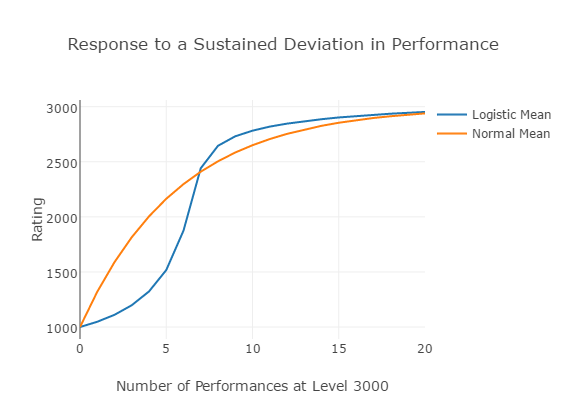
\includegraphics[scale=0.5]{../images/ResponsePlot.png} \end{center}

Had we tried to perform outlier reduction in a memoryless fashion, we would continue to increase the rating by 48 per match, oblivious to the possibility that the player truly did experience a sudden improvement. In Elo-R, the outlier status of a performance is treated as tentative. If later matches support the hypothesis of having improved, the rating will increase by an additional 63 points, followed by over 100 points in each of the third and following matches, as plotted by the blue curve above.

After six consecutive matches with $p_i = 3000$, the rating is 1875 and very unstable (even though $\sigma_i$ is unchanged!). The system is no longer sure which to trust: the extensive history at level 1000, or the smaller number of recent matches at level 3000. Depending on what comes next, the player's rating can very quickly fall toward 1000 or rise toward 3000. However, note that in either case, the change will not overshoot, say to 5000, unless enough new evidence is accumulated at that level. As the $p_i=3000$ streak continues, the seventh match on the blue curve jumps by a whopping 566 points. As the player's rating converges to 3000, the old $p_i = 1000$ data acquires outlier status, thus speeding convergence.

In contrast, while a system such as Codeforces does not compute $p_i$ values in quite in the same way, we can obtain a good approximation by removing outlier reduction from Elo-R, effectively treating the performances to be averaged as normal instead of logistic measurements. This makes the system effectively memoryless, since it turns out that each match simply moves the rating about 16\% closer to the new $p_i$ value, independent of the history. With this change, we obtain the orange curve, which jumps a whopping 320 points at the very first performance. Indeed, there is no limit: if you could find players whose ratings are extremely high, and beat them even once, your rating would take arbitrarily large leaps.

Note that this is not quite true of TopCoder, which incorporates a hack that caps the maximum rating change: if TopCoder's update formula demands too large a change, the cap kicks in. In contrast, Elo-R's cap is a natural and smooth consequence of its update formula and is sensitive to whether a change is charting new territory, or merely confirming a plausible hypothesis. TopCoder does attempt to make the magnitude of its updates sensitive to the amount of fluctuation in a player's history, using a volatility measure, but this measure does not account for the direction of the changes, resulting in the non-monotonicity flaw mentioned above.

Notwithstanding arguments that a high rating ought to properly be earned over multiple matches rather than a single fluke, the other danger is that these observations also hold in reverse: one bad day on Codeforces can seriously damage one's rating and negate several rounds of steady progress. By using heavy-tailed logistic distributions everywhere, Elo-R understands that unusually high or low performances do occasionally occur, and one round in isolation is never a reliable signal.

Interestingly, despite the slow start, the blue curve ultimately converges faster than the orange one. Since Elo-R uses its memory to dynamically adapt its view of potential outliers, it overtakes the orange curve as soon as new evidence outweighs the old hypothesis!

\section{Conclusions}

This paper introduces the Elo-R rating system, which is in part a generalization of the two-player Glicko system, allowing an unbounded number of players. It assumes the players' performances, while potentially hard to quantify directly, can be ranked in a total order. As a natural consequence of some technical modeling assumptions, Elo-R is far more robust to atypical performances than any alternative known to the author.

Applications include many types of sports and video games, as well as programming contests, which presently rely on less rigorously derived models and hacks. The modeling assumptions are best suited to events where the players have minimal targeted interactions against one another, and instead compete individually to score better than rival players in an ongoing array of challenges. For instance, suppose we want to measure a person's skill in traversing obstacle courses, where the course design changes weekly. Completion times are only meaningful on a single course. However, if we treat each course as a match in Elo-R, it becomes possible to quantify and compare the skills of individuals, even if they have never completed the same course together.

\section*{Acknowledgements}

I'm grateful to Daniel Sleator and Dougal Sutherland for discussions that contributed to the inspiration and preparation of this work. In addition, I'd like to thank Mike Mirzayanov for providing a useful case study by publishing the Codeforces rating algorithm.

\bibliographystyle{plain}
\bibliography{Elo}

\end{document}
